
\section{Calibrazione dei rivelatori}
I rivelatori di quasi picco e media devono essere necessariamente calibrati
secondo i valori e le metodologie fornite dalla norma.
La prima metodologia di calibrazione analizzata viene chiamata \textbf{assoluta} (in ampiezza), 
si definisce l'area \textit{IS} dell'impulso con la seguente:
$$ %forula area IS dell'impulso
IS = \int_{-\infty}^{+\infty} v(t) dt
$$

Riferendosi alla tabella sottostante, la calibrazione del rivelatore di \textbf{quasi-picco}
viene effettuata mediante l'analisi della risposta agli impulsi con area
\textit{IS} pari ad \textit{a)}, spettro uniforme almeno fino a \textit{b)}, e
frequenza di ripetizione pari a \textit{c)}, deve essere la stessa (entro \SI{1.5}{\decibel}) di un
segnale sinusoidale non modulato di pari frequenza, avente un'ampiezza
di valore efficace pari a \SI{2}{\milli\volt} ossia \SI{66}{\decibel\micro\volt}.

\begin{center} %tabella parametri calibrazione assoluta quasipico
 \begin{tabular}{|>{\centering}p{4cm}|>{\centering}p{2.8cm}|>{\centering}p{2.8cm}|p{2.8cm}<{\centering}|}
  \hline
    \textbf{Frequency range} & \textbf{a)} \si{\micro\volt\second} & \textbf{b)} \si{\mega\hertz} & \textbf{c)} \si{\hertz} \\ \hline
    \SI{9}{\kilo\hertz} to \SI{150}{\kilo\hertz}     & 13.5  & 0.15 & 25  \\ \hline
    \SI{150}{\kilo\hertz} to \SI{30}{\mega\hertz}    & 0.316 & 30   & 100 \\ \hline
    \SI{30}{\mega\hertz} to \SI{300}{\mega\hertz}    & 0.044 & 300  & 100 \\ \hline
    \SI{300}{\mega\hertz} to \SI{1000}{\mega\hertz}  & 0.044 & 1000 & 100 \\ \hline
 \end{tabular}
\end{center}

Si analizza ora la calibrazione \textbf{relativa} (in frequenza).
Seguendo la curva in figura \ref{fig:calibrazione_relativa} si valuta 
la variazione di \textit{ampiezza} da dare al segale al variare
della frequenza di ripetizione per ottenere sempre la stessa
indicazione di quasi-picco dallo strumento.

\begin{figure}[h] %figura calibrazione relativa quasi-picco
 \centering
 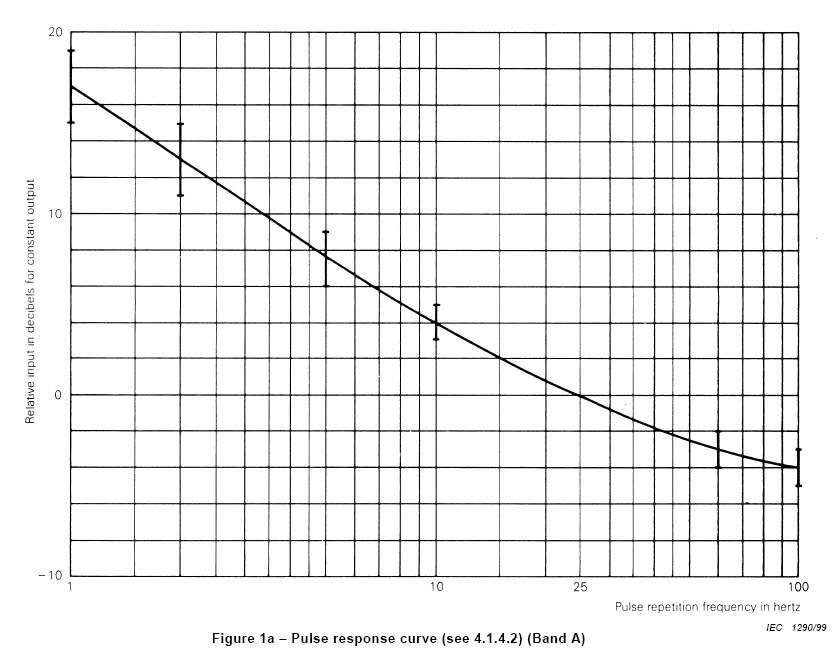
\includegraphics[width=0.7\textwidth]{calibrazione_relativa}
 \caption{Valore del segnale da fornire al variare della frequenza di ripetizione}
 \label{fig:calibrazione_relativa}
\end{figure}

\paragraph{Rilevatore di picco}
Per questo rilevatore viene specificata l'ampiezza di banda a \SI{-6}{\decibel} con
una banda aggiuntiva (Banda E) per segnali superiori a \SI{1}{\giga\hertz}, in questo
caso la banda dell'impulso di riferimento viene calcolata mediante la seguente
$$ %formula B_{imp}
 B_{\text{imp}} = A(t)_{\text{max}} / 2G_0 \cdot IS
$$

I valori per le altre bande sono definiti in tabella:

\begin{center} %tabella parametri banda picco
 \begin{tabular}{|>{\centering}m{5cm}|>{\centering}m{3.2cm}|m{3.2cm}<{\centering}|}
  \hline
    \textbf{Frequency range} & \textbf{Bandwidth $B_6$} & \textbf{Reference BW}  \\ \hline
    \SI{9}{\kilo\hertz}   to \SI{150}{\kilo\hertz}  (A)   & \SI{100}{\hertz}      to \SI{300}{\hertz}      & \SI{200}{\hertz}      \\ \hline
    \SI{150}{\kilo\hertz} to \SI{30}{\mega\hertz}   (B)   & \SI{8}{\kilo\hertz}   to \SI{10}{\kilo\hertz}  & \SI{9}{\kilo\hertz}   \\ \hline
    \SI{30}{\mega\hertz}  to \SI{1000}{\mega\hertz} (C+D) & \SI{100}{\kilo\hertz} to \SI{500}{\kilo\hertz} & \SI{120}{\kilo\hertz} \\ \hline
    \SI{3}{\giga\hertz}   to \SI{18}{\giga\hertz}   (E)   & \SI{300}{\kilo\hertz} to \SI{2}{\mega\hertz}   & \SI{1}{\mega\hertz}   \\ \hline
 \end{tabular}
\end{center}

A differenza delle caratteristiche specifiche del rilevatore di quasi-picco,
per quanto riguarda le \textbf{costanti} di carica e di scarica, viene
definito dalla CISPR il \textit{rapporto minimo fra la costante di scarica e carica
che consente di raggiungere un'indicazione entro il 10\% del valore di picco con un segnale
con frequenza di ripetizione di \SI{1}{\hertz}}
\begin{itemize} % elenco rapporti tra le costanti di carica e scarica picco
 \item [a)] $1.89\cdot10^4$ in banda A   (\SI{9}{\kilo\hertz}   $\sim$ \SI{150}{\kilo\hertz})
 \item [b)] $1.25\cdot10^6$ in banda B   (\SI{150}{\kilo\hertz} $\sim$ \SI{30}{\mega\hertz})
 \item [c)] $1.67\cdot10^7$ in banda C+D (\SI{30}{\mega\hertz}  $\sim$ \SI{1000}{\mega\hertz})
 \item [d)] $1.34\cdot10^8$ in banda D   (\SI{1}{\giga\hertz}   $\sim$ \SI{18}{\giga\hertz})
\end{itemize}

Si definisce inoltre la risposta agli impulsi di area 
pari a $1.4/B_{\text{imp}}$ \si{\milli\volt\second} che deve essere pari a quella
fornita per un segnale sinusoidale di valore efficace \SI{2}{\milli\volt} (\SI{66}{\decibel\micro\volt})

\begin{table}[h] %tabella risposta agli impulsi Picco table generated on tablesgenerator.com
\centering
%\resizebox{\textwidth}{!}{%
\begin{tabular}{|c|c|c|c|c|}
\hline
\multirow{3}{*}{Frequency} & \multirow{3}{*}{\makecell{ IS \\ \si{\milli\volt\second}}} & \multirow{3}{*}{\makecell{$B_{\text{imp}}$\\ \si{\hertz}}} &
\multicolumn{2}{c|}{\multirow{2}{*}{\makecell{Ratio peak/quasi-peak (\si{\decibel})\\ for pulse repetition rate}}} \\
                           &       &        & \multicolumn{2}{c|}{}   \\ \cline{4-5} 
                           &       &        & 25 \si{\hertz}          & 100 \si{\hertz}     \\ \hline
Band A                     & 6.67  & $0.21\cdot10^3$   & 6.1          & $-$                 \\ \hline
Band B                     & $0.148\cdot10^{-3}$       & $9.45\cdot10^3$   & $-$            & 6.6       \\ \hline
Band C + D                 & $0.011\cdot10^{-3}$       & $126.0\cdot10^3$  & $-$            & 12.0      \\ \hline
\end{tabular}%
%}
\end{table}

Come si vede in tabella, il rilevatore di picco viene confrontato con un rilevatore
di quasi-picco già conforme alle norme CISPR.

Anche per quanto riguarda il rilevatore di \textbf{media} viene utilizzata una tabella
con i parametri dell'ampiezza di banda del rivelatore.

\begin{center} %tabella parametri banda media
 \begin{tabular}{|>{\centering}m{5cm}|>{\centering}m{3.2cm}|m{3.2cm}<{\centering}|}
  \hline
    \textbf{Frequency range} & \textbf{Bandwidth $B_6$} & \textbf{Reference BW}  \\ \hline
    \SI{9}{\kilo\hertz}   to \SI{150}{\kilo\hertz}  (A)   & \SI{100}{\hertz}      to \SI{300}{\hertz}      & \SI{200}{\hertz}      \\ \hline
    \SI{150}{\kilo\hertz} to \SI{30}{\mega\hertz}   (B)   & \SI{8}{\kilo\hertz}   to \SI{10}{\kilo\hertz}  & \SI{9}{\kilo\hertz}   \\ \hline
    \SI{30}{\mega\hertz}  to \SI{1000}{\mega\hertz} (C+D) & \SI{100}{\kilo\hertz} to \SI{500}{\kilo\hertz} & \SI{120}{\kilo\hertz} \\ \hline
    \SI{3}{\giga\hertz}   to \SI{18}{\giga\hertz}   (E)   & \SI{300}{\kilo\hertz} to \SI{2}{\mega\hertz}   & \SI{1}{\mega\hertz}   \\ \hline
 \end{tabular}
\end{center}

Per quanto riguarda la calibrazione in ampiezza invece, per impulsi di area pari a 
1.4/n \si{\milli\volt\second} con frequenza di ripetizione pari a n \si{\hertz},
la risposta deve essere pari a quella fornita per un segnale sinusoidale di valore efficace
pari a 2 \si{\milli\volt} (\SI{66}{\decibel\micro\volt}).

\begin{table}[h] %tabella risposta agli impulsi Media (sempre su tablesgenerator.com) Non impazzire con il codice di latex!!!
\centering
\begin{tabular}{|c|c|c|c|c|c|}
\hline
\multirow{3}{*}{Frequency} & \multicolumn{5}{c|}{\multirow{2}{*}{Ratio quasi-peak/average (\si{\decibel}) for pulse repetition rate}} \\
                           & \multicolumn{5}{c|}{}                                                                                 \\ \cline{2-6} 
                           & \SI{25}{\hertz}    & \SI{100}{\hertz}   & \SI{500}{\hertz}   & \SI{1000}{\hertz}  & \SI{5000}{\hertz} \\ \hline
Band A                     & 12.4               &                    &                    &                    &                   \\ \hline
Band B                     &                    & (32.9)             & 22.9               & (17.4)             &                   \\ \hline
Band C + D                 &                    &                    &                    & (38.1)             & 26.3              \\ \hline
\end{tabular}
\end{table}

Le caratteristiche comuni dell'ampiezza di banda permettono ai costruttori degli strumenti
di misura di realizzare un unico filtro a frequenza intermedia con le stesse
caratteristiche per tutte e tre le tipologie di misura.

Il rilevatore di picco rileva sempre l'impulso di ampiezza maggiore, a prescindere
dal numero di impulsi ricevuti, diversamente il quasi-picco è sensibile al numero di impulsi rilevati.
La curva del rivelatore di average invece pesa gli impulsi proporzionalmente alla frequenza.

Il tempo di misura si riferisce alla misura di una \textit{singola} frequenza,
anche in un analizzatore di spettro, il filtro permane per una certa quantità di tempo
sulla singola frequenza. L'intervallo di frequenze si chiama \textbf{span} mentre 
il tempo necessario ad analizzare tutte le frequenze si chiama \textbf{sweep time}.
Lo scan rate è quindi così definito:
$$
 \text{scan rate} = \frac{\text{span}}{\text{sweep time}}
$$
Altro elemento importante nell'analisi spettrale è la \textit{resolution bandwidth}.
Il tempo necessario a ricavare una misura è limitato proprio dal tempo di regime
del filtro intermedio.

Se ad esempio si richiede al rilevatore di picco un tempo di misura
superiore a \SI{100}{\milli\second}, lo strumento effettua comunque una misura
ogni \SI{100}{\milli\second} e restituirà il massimo valore acquisito.
Nel caso del rilevatore di media, se si imposta un tempo di misura superiore
a \SI{100}{\milli\second}, i risultati verranno mediati numericamente con
un convertitore analogico-digitale.

